%%-----------------------------------------------------------------------%%
%%--- Graph Algorithms --------------------------------------------------%%

\chapter{Graph Algorithms}
\label{chap:graph_algorithms}

Graph algorithms have many applications. Suppose you are a salesman
with a product you would like to sell in several cities. To determine
the cheapest travel route from city-to-city, you must effectively
search a graph having weighted edges for the ``cheapest'' route
visiting each city once. Each vertex denotes a city you must visit and
each edge has a weight indicating either the distance from one city to
another or the cost to travel from one city to another.

Shortest path algorithms are some of the most important algorithms in
algorithmic graph theory. We shall examine several in this chapter.


%%-----------------------------------------------------------------------%%
%%--- Graph searching ---------------------------------------------------%%

\section{Graph searching}

This section discusses algorithms for

\begin{itemize}
\item
breadth-first searches,

\item
depth-first searches, and

\item
we explain how these relate to determining a graph's connectivity.
\end{itemize}


%%--- Breadth-first search ----------------------------------------------%%

\subsection{Breadth-first search}

\emph{Breadth-first search} (BFS) is a strategy for running through
the nodes of a graph. Suppose you want to count the number of vertices
(or edges) satisfying a property
$P$. Algorithm~\ref{alg:graph_algorithms:breadth_first_search}
presents a technique for finding the number of vertices satisfying $P$.

\begin{algorithm}[!htpb]
\SetLine
\dontprintsemicolon  % no semicolon at end of pseudocode statements
%% data section
\SetKwInOut{Input}{Input}
\SetKwInOut{Output}{Output}
\SetKwData{Count}{count}
\SetKwData{False}{False}
\SetKwData{True}{True}
%% input/output
\Input{A connected graph $G = (V, E)$ (and, optionally, a starting or
  ``root'' vertex $v_0 \in V$). A property $P$ to be tested.}
\Output{The number of vertices of $G$ satisfying $P$.}
\BlankLine
%% algorithm body
Create a queue $Q$ of ``unseen'' vertices initially containing a
starting vertex $v_0$.\;

Start a list $T$ of ``already seen'' vertices initially empty.\;

$\Count \leftarrow 0$\;

\For{$w \in Q$}{
  Test $w$ for $P$.\;
  \If{$P(w) = \True$}{
    $\Count \leftarrow \Count + 1$\label{abc:step:counter}
  }
  Add all neighbors of $w$ not in $T$ to $Q$.\;
  Remove all ``seen'' vertices $w$ from $Q$.\;
  Add such $w$ to $T$.\;
  \If{$T = V$}{
    \Return \Count
  }
}
\caption{Breadth-first search.}
\label{alg:graph_algorithms:breadth_first_search}
\end{algorithm}

%Algorithm to find a vertex satisfying property P.
%INPUT: Connected graph $G=(V,E)$ and a fixed
%starting vertex $v\in V$.
%OUTPUT:
%True if a vertex is found satisfying P,
%False otherwise.
%1. Start a queue Q containing $v$. Start a
%list of tested vertices, T, initially empty.
%2. For each element w of the queue:
%(a) Test w for P (stop if True).
%(b) Add all neighbors of w not yet tested
%to the queue.
%(c) Remove all tested vertices from the queue
%and add them to T.
%(d) If T=V, stop and return False.

Another version of
Algorithm~\ref{alg:graph_algorithms:breadth_first_search} is where you
are searching the graph for a vertex (or edge) satisfying a certain
property $P$. In that situation, you simply quit at the step where you
increment the counter, i.e. line~7 in
Algorithm~\ref{alg:graph_algorithms:breadth_first_search}. Other
variations are also possible as well.

For the example of the graph in
Figure~\ref{fig:introduction:types_of_walks}, the list of distances
from vertex \verb!a! to any other vertex is
%
\begin{center}
\fontsize{9pt}{9pt}
\selectfont
\tt
\begin{lstlisting}
[['a', 0], ['b', 1], ['c', 2], ['d', 3], ['e', 1], ['f', 2], ['g', 2]]
\end{lstlisting}
\end{center}
%
To create this list,
%
\begin{itemize}
\item
Start at \verb!a! and compute the distance from \verb!a! to itself.

\item
Move to each neighbor of \verb!a!, namely \verb!b! and \verb!e!, and
compute the distance from \verb!a! to each of them.

\item
Move to each ``unseen'' neighbor of \verb!b!, namely just \verb!c!,
and compute the distance from \verb!a! to it.

\item
Move to each ``unseen'' neighbor of \verb!e!, namely just \verb!f!,
and compute the distance from \verb!a! to it.

\item
Move to each ``unseen'' neighbor of \verb!c!, namely just \verb!d!,
and compute the distance from \verb!a! to it.

\item
Move to each ``unseen'' neighbor of \verb!f!, namely just \verb!g!,
and compute the distance from \verb!a! to it.
\end{itemize}

As an example, here is some Sage code which implements BFS to compute
the list distances from a given vertex.
%
\begin{center}
\fontsize{9pt}{9pt}
\selectfont
\tt
\begin{lstlisting}
def graph_distance(G, v0):
    """
    Breadth first search algorithm to find the
    distance from a fixed vertex $v_0$ to any
    other vertex.

    INPUT:
        G - a connected graph
        v0 - a vertex

    OUTPUT:
        D - a list of distances to
            every other vertex

    EXAMPLES:
        sage: G = Graph({1: [2, 4], 2: [1, 4], 3: [2, 6],
                         4: [1, 3], 5: [4, 2], 6: [3, 1]})
        sage: v0 = 1
        sage: graph_distance(G,v0)
        [[1, 0], [2, 1], [3, 2], [4, 1], [5, 2], [6, 1]]
        sage: G = Graph({"a": ["b", "e"], "b": ["c", "e"], \
         "c": ["d", "e"], "d": ["f"], "e": ["f"], "f": ["g"], "g":["b"]})
        sage: v0 = "a"
        sage: graph_distance(G, v0)
        [['a', 0], ['b', 1], ['c', 2], ['d', 3], ['e', 1],
         ['f', 2], ['g', 2]]
        sage: G = Graph({1: [2,3], 2: [1, 3], 3: [2], 4: [5], 5: [6], 6: [5]})
        sage: v0 = 1
        sage: graph_distance(G, v0) # note G is disconnected
        [[1, 0], [2, 1], [3, 1]]
    """
    V = G.vertices()
    Q = [v0]
    T = []
    D = []
    while Q<>[] and T<>V:
        for v in Q:
            if not(v in T):
                D.append([v,G.distance(v0,v)])
            if v in Q:
                Q.remove(v)
            T.append(v)
            T = list(Set(T))
            Q = Q+[x for x in G.neighbors(v) if not(x in T+Q)]
            if T == V:
                break
    D.sort()
    print Q, T
    return D
\end{lstlisting}
\end{center}
%
\begin{exercise}
Using Sage's \verb!shortest_path! method, can you modify the above
function to return a list of shortest paths from $v_0$ to any other
vertex?
\end{exercise}


%%--- Depth-first search ------------------------------------------------%%

\subsection{Depth-first search}

A depth-first search is a type of algorithm that visits each vertex of
a graph, proceeding from vertex-to-vertex in this search but moving
along a spanning tree of that graph.

Suppose you have a normal $8 \times 8$ chess board in front of you,
with a single knight piece on the board. If you can find a sequence of
knight moves which visits each and every square exactly once, then you
will have found a so-called \emph{complete knight tour}.
\index{knight tour}
Naively, how do you find a complete knight tour? Intuitively, you
would make one knight move after another, recording each move to
ensure that you did not step on a square you have already visited,
until you could not make any more moves. It is very, very unlikely
that if do this you will have visited every square exactly once (if
you don't believe me, please try it yourself!). Acknowledging defeat,
at this stage, it might make sense to \emph{backtrack} a few moves and
try again, hoping you will not get ``stuck'' so soon. If you fail
again, try backtracking a few move moves and traverse yet another
path, hoping to make further progress. Repeat this until a compete
tour is found. This is an example of \emph{depth-first search}, also
sometimes called \emph{backtracking}.

Similar to BFS, \emph{depth-first search} (DFS) is an algorithm for
traversing a graph. One starts at a \emph{root vertex} and explores as
\emph{far as possible} along each branch before, if necessary,
backtracking along a new path. It is easier to see what this means in
the case of a rooted tree than for more general graphs, as illustrated
below.
\index{depth-first search}

Suppose you want to count the number of vertices (or edges) satisfying
a property $P$.

\begin{algorithm}[!htpb]
\SetLine
\dontprintsemicolon  % no semicolon at end of pseudocode statements
%% data section
\SetKwInOut{Input}{Input}
\SetKwInOut{Output}{Output}
\SetKwData{Count}{count}
\SetKwData{False}{False}
\SetKwData{True}{True}
%% input/output
\Input{A rooted tree $G = (V, E)$ with  root vertex $v_0 \in V$.}
\Output{\True if $G$ has a vertex satisfying $P$; \False otherwise.}
\BlankLine
%% algorithm body
Create a queue $Q$ of ``child'' vertices of the root $v_0$.\;
Initialize a list $S$ of ``seen'' vertices.\;
$\Count \leftarrow 0$\;
\For{$w \in Q$}{
  Test $w$ for $P$.\;
  \If{$P(w) = \True$}{
    $\Count \leftarrow \Count + 1$
  }
  Add $w$ to $S$.\;
  \If{$S = V$} {
    \Return \Count
  }
}
Call the DFS algorithm iteratively with the rooted subtree having $w$
and all its children as vertices and $w$ as the rooted vertex.
\caption{Depth-first search.}
\label{alg:graph_algorithms:depth_first_search}
\end{algorithm}

In the case of a graph, you can modify
Algorithm~\ref{alg:graph_algorithms:depth_first_search} to a so-called
iterative DFS. This modification applies DFS repeatedly with an
increasing depth of search at each step, until the diameter of the
graph is reached and all vertices are seen.

\subsection{Connectivity of a graph}

% This subsection is on how the above algorithms can be used
% to determine a graph's connectivity.


%%-----------------------------------------------------------------------%%
%%--- Dijkstra's algorithm ----------------------------------------------%%

\section{Dijkstra's algorithm}

See Dijkstra~\cite{Dijkstra1959}, section~24.3 of
Cormen~et~al.~\cite{CormenEtAl2001}, and section~12.6 of Berman and
Paul~\cite{BermanPaul1997}.

Dijkstra's algorithm, discovered by E.~Dijkstra in 1959, is a graph
search algorithm that solves the single-source shortest path problem
for a graph with non-negative edge weights. For example, if the
vertices of a weighted graph represent cities and edge weights
represent distances between pairs of cities connected by a direct
road, Dijkstra's algorithm can be used to find the shortest route from
a fixed city to all other cities.

%It is remarkable that, at the present state of knowledge, given two
%distinct vertices $v, w$ of a graph $G=(V,E)$, the fastest algorithm
%determining a shortest path from $v$ to $w$ appears to be no faster (in general)
%than the fastest algorithm determining a shortest path from $v$ to
%\emph{any} other vertex of $G$.

Let $G = (V,E)$ be a graph with non-negative edge weights, $w(e)$ for
$e \in E$. Fix a start or source vertex $v_0 \in V$. The
\emph{length of a path} $P$ from $v \in V$ to $w \in V$ is the sum of
the edge weights for each edge in the path $P$, denoted
$\delta(P)$. We write $\delta(v,w)$ for the smallest value of
$\delta(P)$ for all paths $P$ from $v$ to $w$.
\index{path length}

Dijkstra's algorithm performs a number of steps, basically one step
for each vertex in $V$. We partition the vertex set $V$ into two
subsets: the set $F$ of vertices where we have found the shortest path
to $v_0$; and the ``queue'' $Q$ where we do not yet know for sure the
shortest path to $v_0$. The vertices $v \in F$ are labeled with
$\delta(v, v_0)$. The vertices $v \in Q$ are labeled with a temporary
label $L(v)$. This temporary label can be either $\infty$ if no path
from $v$ to $v_0$ has yet been examined, or an upper bound on
$\delta(v, v_0)$ obtained by computing $\delta(P)$ for a path $P$ from
$v$ to $v_0$ which has been found (but may not be the shortest path).

\begin{algorithm}[!htpb]
\SetLine
\dontprintsemicolon  % no semicolon at end of pseudocode statements
%% data section
\SetKwInOut{Input}{Input}
\SetKwInOut{Output}{Output}
\SetKwData{Count}{count}
\SetKwData{False}{False}
\SetKwData{True}{True}
%% input/output
\Input{A connected graph $G = (V, E)$ having non-negative edge weights
and a starting vertex $v_0 \in V$. }
\Output{A shortest path from $v_0$ to an vertex in $V$.}
\BlankLine
%% algorithm body
Create a queue $Q$ of ``unseen'' vertices initially being
all of $V$.\;

Start a list $F$ of ``already seen'' vertices initially empty.\;

Initialize labels $L(v_0) = 0$ and $L(v) = \infty$ for all
$v \in V$ with $v \neq v_0$.\;

Find $v \in Q$ for which $L(v)$ is finite and minimum.\;

\eIf{\emph{no such $v$ exists}}{
  \Return
}{
  Label $v$ with the distance $\delta(v, v_0) = L(v)$.\;
  Add $v$ to $F$.\;
  Remove $v$ from $Q$.\;
  \If{$F = V$}{
    \Return
  }
}

\For{\emph{$w \in Q$ such that $w$ is adjacent to $v$}}{
  Replace $L(w)$ by $\min(L(w),\, L(v) + wt(v,w))$.\;
  Go to step 4.
}
\caption{Dijkstra's algorithm.}
\label{alg:graph_algorithms:dijkstra}
\end{algorithm}

\begin{figure}[!htbp]
\centering
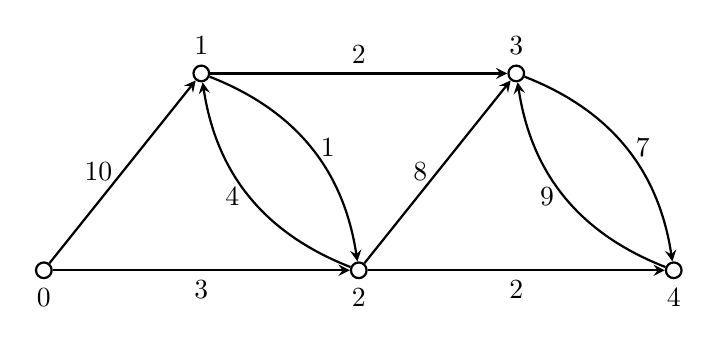
\begin{tikzpicture}
[nodedecorate/.style={shape=circle,inner sep=2pt,draw,thick},%
  arrowdecorate/.style={->,>=stealth,thick}]
% nodes or vertices
\node (0) at (0,0) [nodedecorate] {};
\node [below] at (0.south) {$0$};
\node (2) at (4,0) [nodedecorate] {};
\node [below] at (2.south) {$2$};
\node (4) at (8,0) [nodedecorate] {};
\node [below] at (4.south) {$4$};
\node (1) at (2,2.5) [nodedecorate] {};
\node [above] at (1.north) {$1$};
\node (3) at (6,2.5) [nodedecorate] {};
\node [above] at (3.north) {$3$};
% edges or lines
\path
(0) edge[arrowdecorate] node[left]{$10$} (1)
(0) edge[arrowdecorate] node[below]{$3$} (2)
(1) edge[arrowdecorate,bend left] node[right]{$1$} (2)
(1) edge[arrowdecorate] node[above]{$2$} (3)
(2) edge[arrowdecorate,bend left] node[left]{$4$} (1)
(2) edge[arrowdecorate] node[left]{$8$} (3)
(2) edge[arrowdecorate] node[below]{$2$} (4)
(3) edge[arrowdecorate,bend left] node[right]{$7$} (4)
(4) edge[arrowdecorate,bend left] node[left]{$9$} (3);
\end{tikzpicture}
\caption{Searching a weighted digraph using Dijkstra's algorithm.}
\label{fig:graph_algorithms:Dijkstra_algorithm_digraph}
\end{figure}
%sage: M = matrix([[0,10,3,0,0],[0,0,1,2,0],[0,4,0,8,2],[0,0,0,0,7],[0,0,0,9,0]])
%sage: D = DiGraph(M, format="weighted_adjacency_matrix")
%sage: D.plot(edge_labels=True, graph_border=True).show()

\begin{table}[!htbp]
\centering
\begin{tabular}{|ccccc|} \hline
$v_0$         & $v_1$         & $v_2$         & $v_3$         & $v_4$ \\\hline\hline
\underline{0} & $\infty$      & $\infty$      & $\infty$      & $\infty$ \\
              & 10            & \underline{3} & $\infty$      & $\infty$ \\
              & 7             &               & 11            & \underline{5} \\
              & \underline{7} &               & 11            & \\
              &               &               & \underline{9} & \\\hline
\end{tabular}
\caption{Stepping through Dijkstra's algorithm.}
\label{tab:graph_algorithms:working_through_Dijkstra_algorithm}
\end{table}

\begin{example}
Apply Dijkstra's algorithm to the graph in
Figure~\ref{fig:graph_algorithms:Dijkstra_algorithm_digraph}.
\end{example}

\begin{proof}[Solution]
Dijkstra's algorithm applied to the graph in
Figure~\ref{fig:graph_algorithms:Dijkstra_algorithm_digraph} yields
Table~\ref{tab:graph_algorithms:working_through_Dijkstra_algorithm}. The
steps below explain how this table is created.
%
\begin{enumerate}
\item
Start at $v_0$, let $Q = V$ and $F = \emptyset$. Initialize the labels
$L(v)$ to be $\infty$ for all $v \neq v_0$. This is the first row of
the table. Take the vertex $v_0$ out of the queue.

\item
Consider the set of all adjacent nodes to $v_0$. Replace the labels in
the first row by the weights of the associated edges. Underline the
smallest one and take its vertex (i.e. $v_2$) out of the queue. This
is the second row of the table.

\item
Consider the set of all nodes $w$ which are adjacent to $v_2$. Replace
the labels in the second row by $\min(L(w),\, L(v_2) + wt(v_2, w))$.
Underline the smallest one and take its vertex (i.e. $v_4$) out of the
queue. This is the third row of the table.

\item
Finally, start from $v_4$ and find the path to the remaining vertex
$v_3$ in $Q$. Take the smallest distance from $v_0$ to $v_3$. This is
the last row of the table.
\end{enumerate}
\end{proof}

\begin{exercise}
Dijkstra's algorithm applied to the graph in
Figure~\ref{fig:graph_algorithms:Dijkstra_directed_house_graph}
results in
Table~\ref{tab:graph_algorithms:another_walkthrough_Dijkstra}. Verify
the steps to create this table.
\end{exercise}

\begin{figure}[!htbp]
\centering
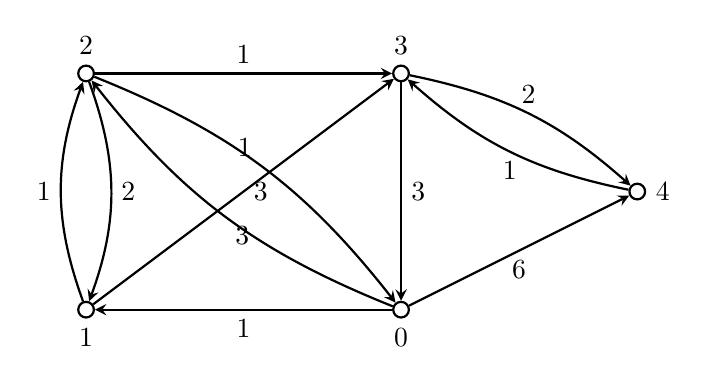
\begin{tikzpicture}
[nodedecorate/.style={shape=circle,inner sep=2pt,draw,thick},%
  arrowdecorate/.style={->,>=stealth,thick}]
% nodes or vertices
\node (0) at (4,0) [nodedecorate] {};
\node [below] at (0.south) {$0$};
\node (1) at (0,0) [nodedecorate] {};
\node [below] at (1.south) {$1$};
\node (2) at (0,3) [nodedecorate] {};
\node [above] at (2.north) {$2$};
\node (3) at (4,3) [nodedecorate] {};
\node [above] at (3.north) {$3$};
\node (4) at (7,1.5) [nodedecorate] {};
\node [right] at (4.east) {$4$};
% edges or lines
\path
(0) edge[arrowdecorate] node[below]{$1$} (1)
(0) edge[arrowdecorate,bend left=15] node[below right]{$3$} (2)
(0) edge[arrowdecorate] node[below]{$6$} (4)
(1) edge[arrowdecorate,bend left=20] node[left]{$1$} (2)
(1) edge[arrowdecorate] node[right]{$3$} (3)
(2) edge[arrowdecorate,bend left=15] node[above left]{$1$} (0)
(2) edge[arrowdecorate,bend left=20] node[right]{$2$} (1)
(2) edge[arrowdecorate] node[above]{$1$} (3)
(3) edge[arrowdecorate] node[right]{$3$} (0)
(3) edge[arrowdecorate,bend left=15] node[above]{$2$} (4)
(4) edge[arrowdecorate,bend left=15] node[below]{$1$} (3);
\end{tikzpicture}
\caption{Searching a directed house graph using Dijkstra's algorithm.}
\label{fig:graph_algorithms:Dijkstra_directed_house_graph}
\end{figure}
%sage: M = matrix([[0,1,3,0,6],[0,0,1,3,0],[1,2,0,1,0],[3,0,0,0,2],[0,0,0,1,0]])
%sage: D = DiGraph(M, format="weighted_adjacency_matrix")
%sage: D.plot(edge_labels=True, graph_border=True).show()

\begin{table}[!htbp]
\centering
\begin{tabular}{|ccccc|} \hline
$v_0$         & $v_1$         & $v_2$         & $v_3$         & $v_4$ \\\hline\hline
\underline{0} & $\infty$      & $\infty$      & $\infty$      & $\infty$ \\
              & \underline{1} & 3             & $\infty$      & 6 \\
              &               & \underline{2} & 4             & 6 \\
              &               &               & \underline{3} & 6 \\
              &               &               &               & \underline{5} \\\hline
\end{tabular}
\caption{Another walk-through of Dijkstra's algorithm.}
\label{tab:graph_algorithms:another_walkthrough_Dijkstra}
\end{table}


%%-----------------------------------------------------------------------%%
%%--- Bellman-Ford algorithm --------------------------------------------%%

\section{Bellman-Ford algorithm}

See section~24.1 of Cormen~et~al.~\cite{CormenEtAl2001}, and
section~8.5 of Berman and Paul~\cite{BermanPaul1997}.

The Bellman-Ford algorithm computes single-source shortest paths in a
weighted graph or digraph, where some of the edge weights may be
negative. Instead of the ``greedy'' approach that Dijkstra's algorithm
took, i.e. searching for the ``cheapest'' path, the Bellman-Ford
algorithm searches over all edges and keeps track of the shortest one
found as it searches.

The implementation below takes in a graph or digraph, and creates two
Python dictionaries \verb!dist! and \verb!predecessor!, keyed on the
list of vertices, which store the distance and shortest
paths. However, if a negative weight cycle exists~(in the case of a
digraph), then an error is raised.

\begin{center}
\fontsize{9pt}{9pt}
\selectfont
\tt
\begin{lstlisting}
def bellman_ford(Gamma, s):
    """
    Computes the shortest distance from s to all other vertices in Gamma.
    If Gamma has a negative weight cycle, then return an error.

    INPUT:

    - Gamma -- a graph.
    - s -- the source vertex.

    OUTPUT:

    - (d,p) -- pair of dictionaries keyed on the list of vertices,
      which store the distance and shortest paths.

    REFERENCE:

    http://en.wikipedia.org/wiki/Bellman-Ford_algorithm
    """
    P = []
    dist = {}
    predecessor = {}
    V = Gamma.vertices()
    E = Gamma.edges()
    for v in V:
        if v == s:
            dist[v] = 0
        else:
            dist[v] = infinity
        predecessor[v] = 0
    for i in range(1, len(V)):
        for e in E:
            u = e[0]
            v = e[1]
            wt = e[2]
            if dist[u] + wt < dist[v]:
                dist[v] = dist[u] + wt
                predecessor[v] = u
    # check for negative-weight cycles
    for e in E:
        u = e[0]
        v = e[1]
        wt = e[2]
        if dist[u] + wt < dist[v]:
            raise ValueError("Graph contains a negative-weight cycle")
    return dist, predecessor
\end{lstlisting}
\end{center}

Here are some examples.

\begin{center}
\fontsize{9pt}{9pt}
\selectfont
\tt
\begin{lstlisting}
sage: M = matrix([[0,1,4,0], [0,0,1,5], [0,0,0,3], [0,0,0,0]])
sage: G = Graph(M, format="weighted_adjacency_matrix")
sage: bellman_ford(G, G.vertices()[0])
  {0: 0, 1: 1, 2: 2, 3: 5}
\end{lstlisting}
\end{center}
%
The plot of this graph is given in
Figure~\ref{fig:graph_algorithms:Bellman_Ford_example}.

\begin{figure}[!htbp]
\centering
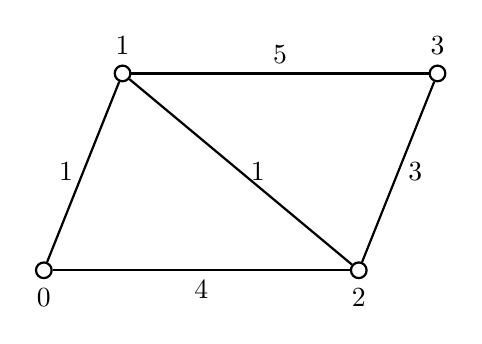
\begin{tikzpicture}
[nodedecorate/.style={shape=circle,inner sep=2pt,draw,thick},%
  linedecorate/.style={-,thick}]
% nodes or vertices
\node (0) at (0,0) [nodedecorate] {};
\node [below] at (0.south) {$0$};
\node (2) at (4,0) [nodedecorate] {};
\node [below] at (2.south) {$2$};
\node (1) at (1,2.5) [nodedecorate] {};
\node [above] at (1.north) {$1$};
\node (3) at (5,2.5) [nodedecorate] {};
\node [above] at (3.north) {$3$};
% edges or lines
\path
(0) edge[linedecorate] node[left]{$1$} (1)
(0) edge[linedecorate] node[below]{$4$} (2)
(1) edge[linedecorate] node[right]{$1$} (2)
(1) edge[linedecorate] node[above]{$5$} (3)
(2) edge[linedecorate] node[right]{$3$} (3);
\end{tikzpicture}
\caption{Shortest paths in a weighted graph using the Bellman-Ford
  algorithm.}
\label{fig:graph_algorithms:Bellman_Ford_example}
\end{figure}
%sage: M = matrix([[0,1,4,0],[0,0,1,5],[0,0,0,3],[0,0,0,0]])
%sage: G = Graph(M, format = "weighted_adjacency_matrix")
%sage: G.plot(graph_border=True, edge_labels=True).show()

The following example illustrates the case of a negative-weight cycle.

\begin{center}
\fontsize{9pt}{9pt}
\selectfont
\tt
\begin{lstlisting}
sage: M = matrix([[0,1,0,0],[1,0,-4,1],[1,1,0,0],[0,0,1,0]])
sage: G = DiGraph(M, format = "weighted_adjacency_matrix")
sage: bellman_ford(G, G.vertices()[0])
---------------------------------------------------------------------------
...
ValueError: Graph contains a negative-weight cycle
\end{lstlisting}
\end{center}
%
The plot of this graph is given in
Figure~\ref{fig:graph_algorithms:Bellman_Ford_negative_weights}.

\begin{figure}[!htbp]
\centering
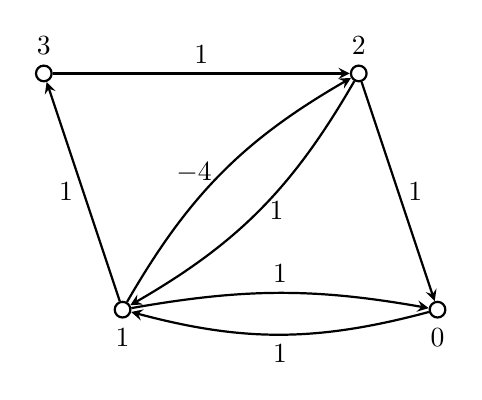
\begin{tikzpicture}
[nodedecorate/.style={shape=circle,inner sep=2pt,draw,thick},%
  arrowdecorate/.style={->,>=stealth,thick}]
% nodes or vertices
\node (0) at (5,0) [nodedecorate] {};
\node [below] at (0.south) {$0$};
\node (1) at (1,0) [nodedecorate] {};
\node [below] at (1.south) {$1$};
\node (2) at (4,3) [nodedecorate] {};
\node [above] at (2.north) {$2$};
\node (3) at (0,3) [nodedecorate] {};
\node [above] at (3.north) {$3$};
% edges or lines
\path
(0) edge[arrowdecorate,bend left=15] node[below]{$1$} (1)
(1) edge[arrowdecorate,bend left=10] node[above]{$1$} (0)
(1) edge[arrowdecorate,bend left=15] node[left]{$-4$} (2)
(1) edge[arrowdecorate] node[left]{$1$} (3)
(2) edge[arrowdecorate] node[right]{$1$} (0)
(2) edge[arrowdecorate,bend left=15] node[right]{$1$} (1)
(3) edge[arrowdecorate] node[above]{$1$} (2);
\end{tikzpicture}
\caption{Searching a digraph with negative weight using the
  Bellman-Ford algorithm.}
\label{fig:graph_algorithms:Bellman_Ford_negative_weights}
\end{figure}
%sage: M = matrix([[0,1,0,0],[1,0,-4,1],[1,1,0,0],[0,0,1,0]])
%sage: G = Graph(M, format = "weighted_adjacency_matrix")
%sage: G.plot(graph_border=True, edge_labels=True).show()


%%-----------------------------------------------------------------------%%
%%--- Floyd-Warshall algorithm ------------------------------------------%%

\section{Floyd-Warshall algorithm}

See section~25.2 of Cormen~et~al.~\cite{CormenEtAl2001}, and section
14.4 of Berman and Paul~\cite{BermanPaul1997}.


%%-----------------------------------------------------------------------%%
%%--- Johnson's algorithm -----------------------------------------------%%

\section{Johnson's algorithm}

See section~25.3 of Cormen~et~al.~\cite{CormenEtAl2001} and
Johnson~\cite{Johnson1977}.
